\chapter{Lösungsansätze}
    Hier ein anderes Kapitel
    Viele Zitate: \cite{patterson} \cite{krizhevsky} \cite{matlab} \cite{pitts} \cite{lawrence} \cite{miesbach}
    \section{Elasticsearch vs. DynamoDB}
        
        The most important thing about Elasticsearch is that Elasticsearch supports full text search and that makes it different froms the normal databases, which are very much black and white, we just store stuff and retrieve it. In Full text search we look more for the concept, not a specific word in singular or in plural but we are looking for the concept or the meaning, which is very complicated to achieve with the normal databases for many reasons: building complicated queries, much more computing time by searching, long time for getting the response and by returning the result and not very performant like with Elasticsearch.
        
        Common Databases are focusing on how to store the data comparing to Elasticsearch that allows us to make sense of our data, explore them and be able to ask questions on the data in a simple way without writing complicated Query.
        Elasticsearch give us the ability to make data exploration, to go ahead and ask questions on the saved data and get results in milliseconds and be ready to visulise and make analytics on them.
               
        \subsection{Subsection}
            \begin{figure}[h]
                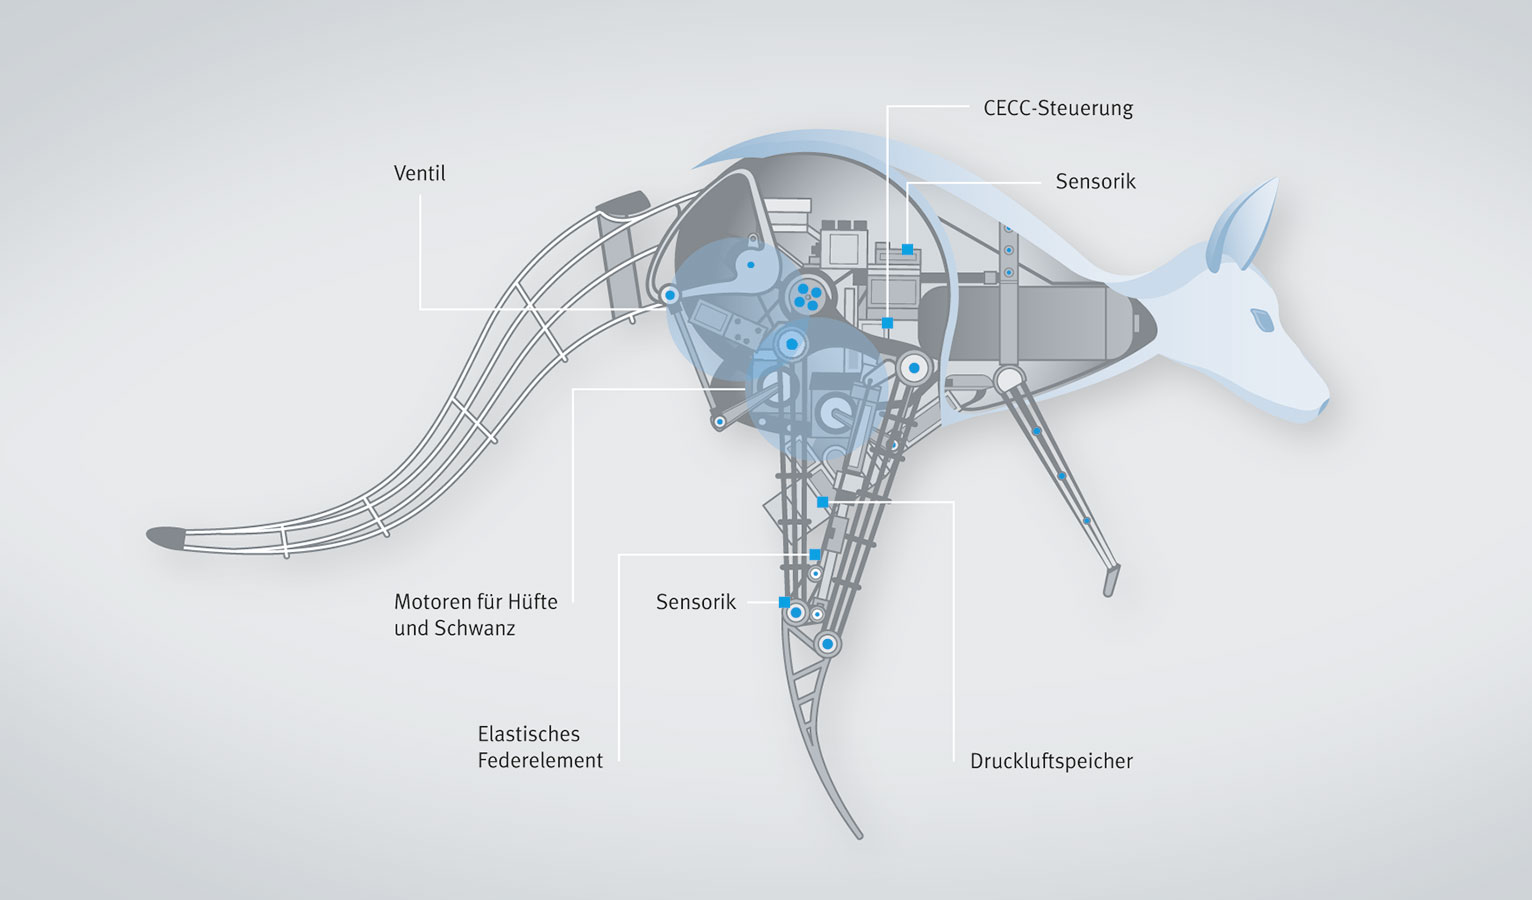
\includegraphics[scale=0.2]{Abbildungen/Kapitel2/Kangoroo.png}
                \centering
                \caption{Ein Kangoroo}
                \label{Abb:Kangoroo}   
            \end{figure}  
             \begin{table}[h]
                \begin{tabular}{ccc}
                      \hline
                      Spalte1 & Spalte2 & Spalte3\\                      
                      \hline
                      1 & 2 & 3\\
                      \hline
                \end{tabular}
                \centering
                \caption{Eine Tabelle}
                \label{Tab:Tabelle1}
            \end{table}
 
        
        
    \section{Kibana und JavaFx}
        Eine Subsection
        \newpage
        Eine neue Seite
        \newpage 
        Noch eine neue Seite
        \newpage    
        und noch eine neue Seite